\section{Interfacce neurali per il monitoraggio dello stato mentale}
Un' interfaccia neurale, nota anche con il termine inglese {\bf Brain-computer interface} (\emph{BCI}), è un mezzo di comunicazione diretto tra un cervello (o più in generale parti funzionali del sistema nervoso centrale) ed un dispositivo esterno quale ad esempio un computer \cite{bci}.\newline
Il dispositivo campiona l’attività cerebrale attraverso tecnologie quali l'elettroencefalogramma (EEG), la spettroscopia funzionale nel vicino infrarosso (fNIRS), ecc...\newline
L'attività cerebrale campionata viene quindi codificata in una forma comprensibile dal calcolatore.\newline
A questo punto i dati ottenuti vengono elaborati da algoritmi il quale scopo è trarre delle metriche che esprimano in modo comprensibile un aspetto cognitivo ricercato (come ad esempio il carico cognitivo visto nella sezione precedente).\newline
\begin{figure}[H]
  \centering
  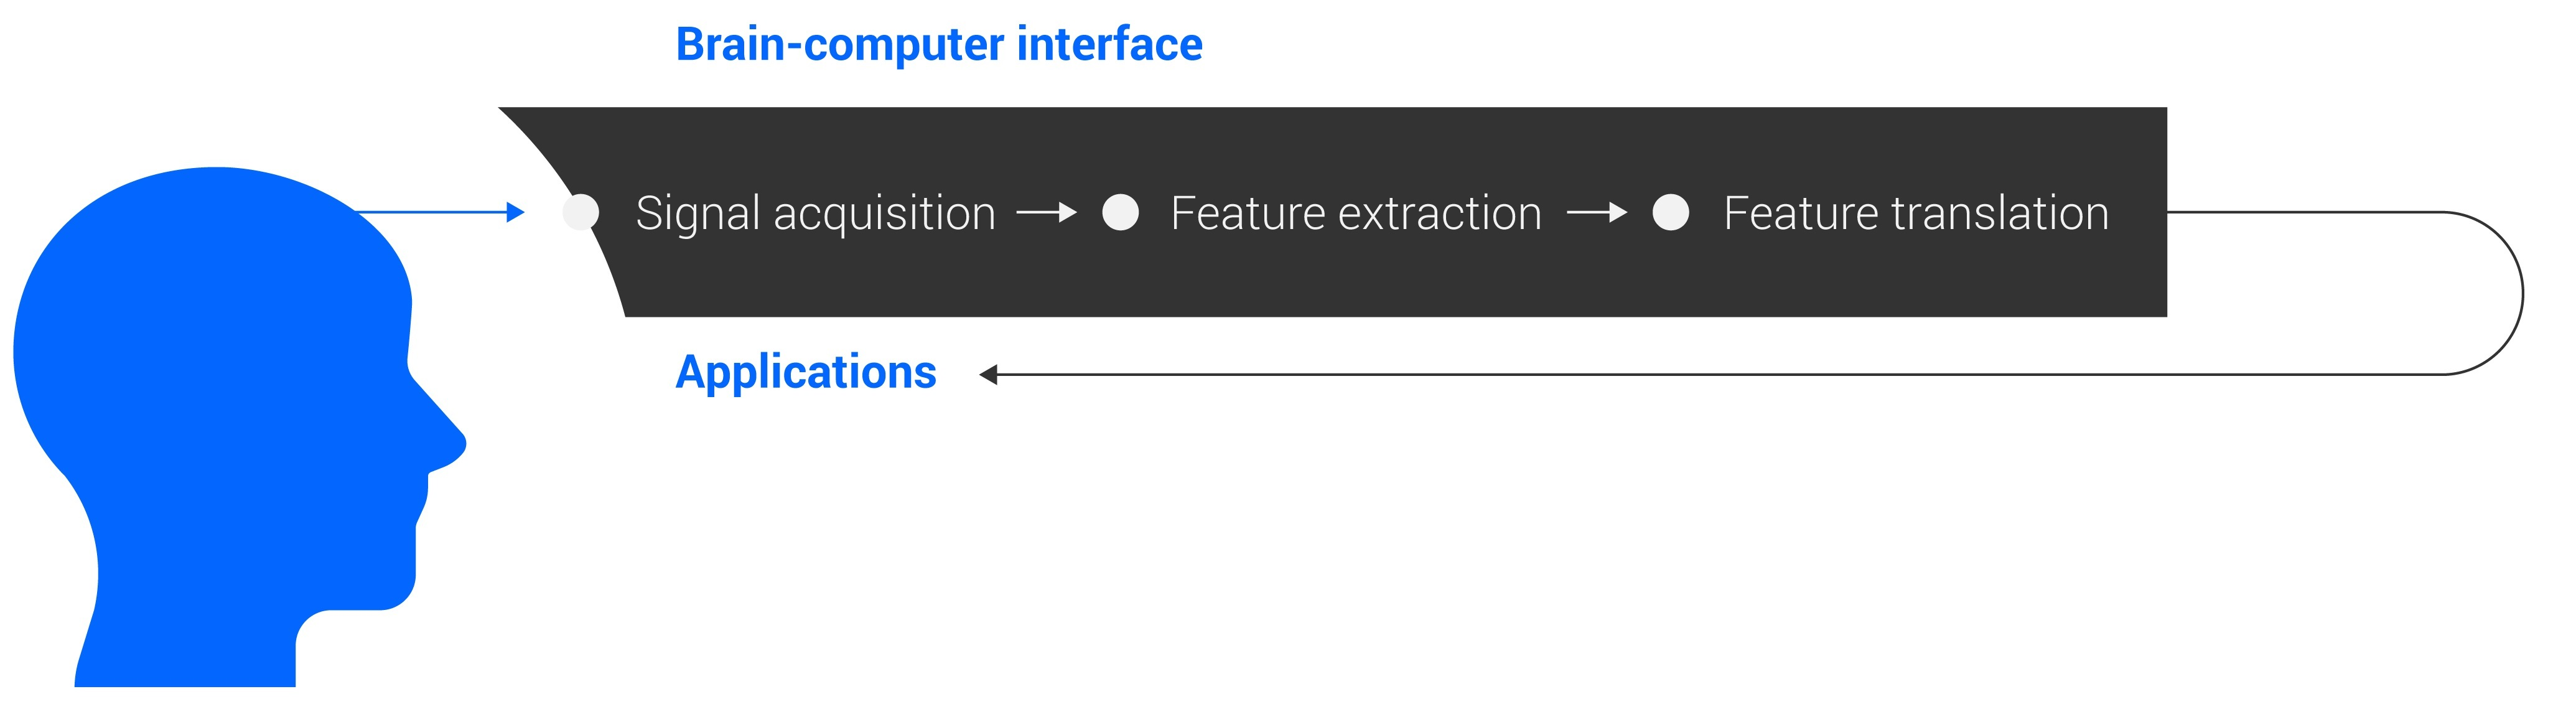
\includegraphics[width=1.0\textwidth]{img/BCI.jpg}
  \caption{Funzionamento ad alto livello di una BCI}
\end{figure}
\noindent Il primo obiettivo che portò alla concezione e realizzazione di BCI fu fornire a persone con disabilità canali di comunicazione o controllo di dispositivi esterni.\newline
Sistemi di questo tipo però rimangono confinati in un contesto medico per due importanti motivazioni:
\begin{itemize}
  \item \emph{Alta specificità delle feature ricercate}
  \item \emph{Hardware costoso ed ingombrante}
\end{itemize}
Nell'ultimo decennio i ricercatori hanno cominciato a prendere in considerazione l'utilizzo delle BCI in contesti che coinvolgano soggetti sani.\newline
Il significato del termine BCI si è dunque evoluto nel tempo; inizialmente il termine si riferiva solamente alla traduzione dell'intento di un utente per attuare una risposta nel mondo fisico.\newline

\noindent Oggi invece il termine si è espanso fino a comprendere il monitoraggio dello stato mentale ed emotivo di un individuo. Questo nuovo tipo di BCI è stato denominato {\bf passive Brain-computer interface} (\emph{pBCI}) \cite{pbci}.\newline
Negli ultimi anni le pBCI sono migliorate incredibilmente in termini di affidabilità, usabilità e contesti di applicazione.\newline
Sono state pubblicate grandi quantità di ricerche riguardanti il potenziale delle pBCI; tuttavia, la maggior parte dei lavori e test è stata condotta in ambiente di laboratorio o comunque ambienti altamente controllati.\newline
